\documentclass[a4paper]{article}

\usepackage[utf8]{inputenc}
\usepackage{hyperref}
\usepackage{graphicx}
\usepackage[section]{placeins}

\addtolength{\textheight}{1cm}
\addtolength{\voffset}{-1cm}
\addtolength{\textwidth}{2cm}
\addtolength{\hoffset}{-1cm}

\graphicspath{{figs/}}
\newcommand{\etd}{EISCAT\_3D}

\title{Prototype DIRAC Web Portal for EISCAT data --- Step by step instructions}
\author{Carl-Fredrik Enell, EISCAT Scientific Association}

\begin{document}
\maketitle{}

\section{Introduction and history}
\label{sec:intro}

EGI (\url{http://www.egi.eu}) is a federated e-Infrastructure set up
to provide advanced computing services for research and innovation.
The Horizon 2020 EINFRA-1-2014 project EGI-Engage supported a number
of competence centres (CCs) for research infrastructures. In this
framework, the CC for \etd{} started to develop a data search and
analysis portal for the future users of \etd{}.

Several services developed by EGI, as well as the related Horizon 2010
projects Indigo DataCloud and EUDAT \url{http://www.eudat.eu}, are now
part of the European Open Science Cloud Hub (EOSC-Hub),
\url{http://www.eosc-hub.eu}, a currently running project funded by
the Horizon 2020 research and innovation programme under grant
agreement No~777536.

Thus, the development initiated in the EGI-Engage CC is continued in
the EOSC-Hub CC for \etd{}. Partners in this project are EISCAT HQ,
Sweden, CNRS-IN2P3, France, and CSC in Finland.

\subsection{DIRAC}
\label{sec:dirac}

The \etd{} competence centre aims at developing the \etd{} user
portal, which is to be the primary interface through which users will
browse, download and analyse \etd{} data.  We chose to work closely
with the developers of the Distributed Infrastructure with Remote
Agent Control (DIRAC) project, \url{http://diracgrid.org}, which was
originally developed for distributing data from the LHCb project at
CERN. DIRAC is an interware, mostly written in Python, that provides
command-line, web and API interfaces to grid computing and storage
resources. The major task of the \etd{} CC so far has been to
implement a prototype DIRAC portal for legacy EISCAT data, i.e. lag
profile data (time-averaged spectral data in the autocorrelation
domain). These data are stored in a Matlab version 4 compatible format
at EISCAT HQ and indexed in a MySQL database.


Detailed user and administrator instructions for DIRAC can be found at
\url{https://dirac.readthedocs.io/en/latest/UserGuide/index.html}. It
is highly recommended to read the user instructions carefully to
obtain a good understanding of what DIRAC can do.

\subsection{Layout of the EISCAT DIRAC service}
\label{sec:eiscat-dirac}

 
The prototype EISCAT DIRAC portal comprises the required functions for
user authentication, data search, and job submission to computing
resources at CSC.

\begin{description}

\item[Virtual organisation membership service (VOMS)] User access to the
  EISCAT DIRAC portal is managed through membership in groups in the
  EGI virtual organisation (VO) \textbf{eiscat.se}.  

  The VOMS used by EGI is called Perun and runs
  at Cesnet, accessible to VOMS managers through a web GUI at
  \url{https://perun.cesnet.cz}

\item[Storage element] Access to storage in DIRAC is handled by the
  storage element (SE) server. This is a Python program and this
  project uses an instance that runs on server at EISCAT
  Headquarters. It reads and serves data files from a top level
  directory, where presently data directories from 1981--1983, 2007
  (IPY) and 2011--2019 are linked from the main storage server.

\item[File catalogue] This is a database of files available on the storage element, and their metadata.  It runs on EGI resources at Cyfronet
  (\url{http://www.cyfronet.krakow.pl}) and allows users
  to list and search the data with a command-line client and the file
  catalogue application in the web portal.  

  The file catalogue is updated by a Python script that runs monthly
  (from cron) on the DIRAC server at EISCAT Headquarters. This script
  reads metadata from the MySQL database at EISCAT, as available at
  \url{https://www.eiscat.se/schedule/schedule.cgi} by selecting
  Archived data.

\item[Web interface] A web interface is the main point of access for
  users. It also runs at Cyfronet and is accessible at
  \url{https://dirac.egi.eu:9443/DIRAC/}. 

  This web interface presents the user with a GUI environment
  (Fig.~\ref{fig:portal}) which has applications for file catalogue
  search, job submission, and more.

\end{description}
\begin{figure}[htb]
  \centering
  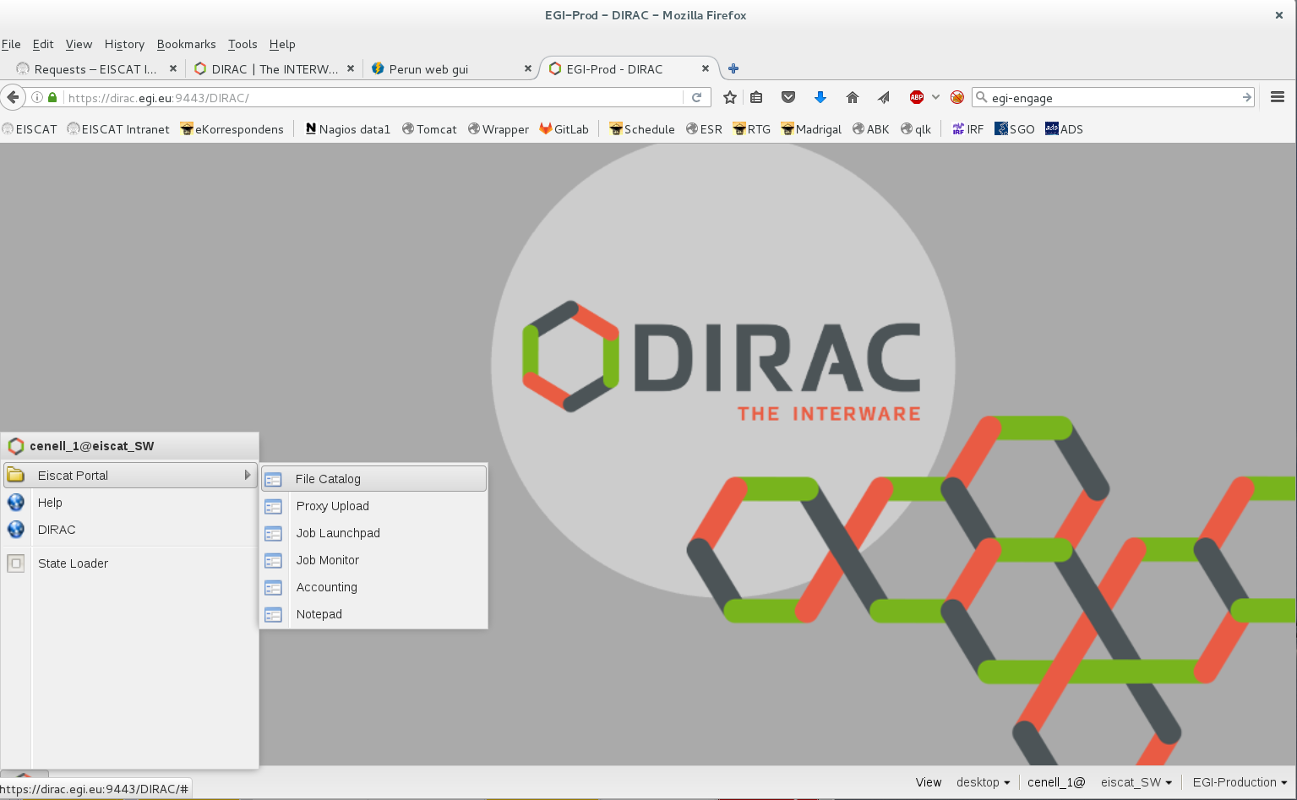
\includegraphics[width=1.0\linewidth]{dirac-gui-desktop}
  \caption{The DIRAC web GUI}
  \label{fig:portal}
\end{figure}

\section{Accessing the \etd{} DIRAC portal}
\label{sec:access}

Access to data in DIRAC requires user authentication and access
authorisation through membership in one ore more groups in the Virtual
Organisation (VO) eiscat.se.

For user authentication two options are implemented: X.509 certificate
authentication and authentication with the EGI Checkin service.
Certificate authentication is the most mature system. However, this has
turned out to be unknown to most EISCAT users, even those who in
principle have access to certificate authorities, and thus a detailed
description follows here. For instructions on EGI Checkin authentication,
skip to Sect.~\ref{sec:checkin-auth} below.


\subsection{Certificate authentication}
\label{sec:cert-auth}


\subsubsection{Get a certificate}
\label{sec:get-certificate}

Skip this section if you already have a Grid Premium type X.509 certificate. In this case it should be installed in your web browser and exportable from there.

\begin{enumerate}


\item Log in to your certificate authority. At least for EISCAT users
  in the Nordic region, this is usually Digicert. Browse to
  \url{https://www.digicert.com/sso/} using a compliant
  browser. Firefox, MS Internet Explorer and Safari should all work,
  but Google Chrome and MS Edge were not compatible when last tried
  (this may change).

  On the first page shown you will have to type in the name of your
  identity provider, i.e. your university or
  institute. Fig.~\ref{fig:idp} shows what this looks like for the
  author, whose identity provider is the Swedish Institute of Space
  Physics. This will redirect you to a login page where you should be
  able to log in with the user credentials of your organisation. In
  many cases this will be the same name and password that you use for
  your university email and internal web pages.

  \begin{figure}[htb]
    \centering
    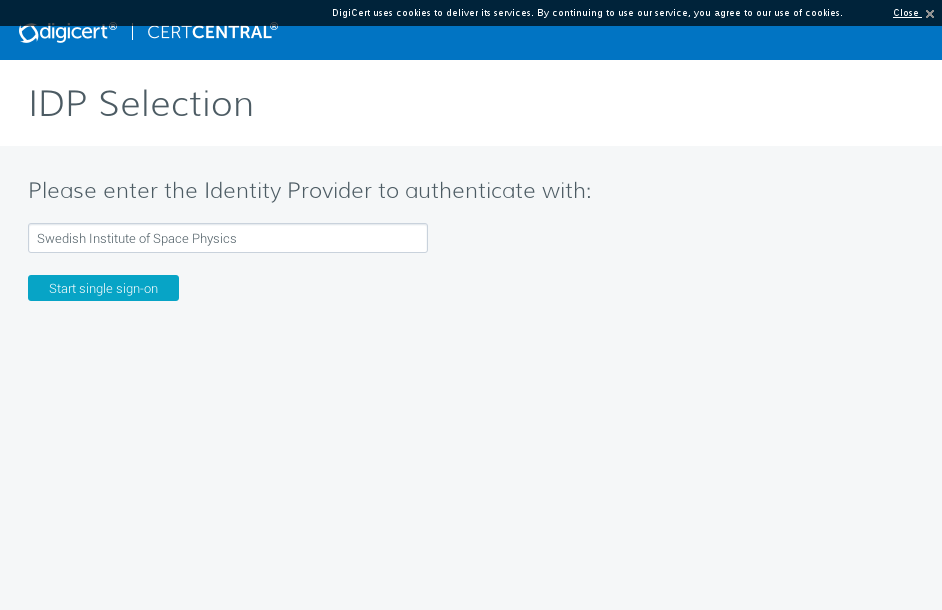
\includegraphics[width=1.0\linewidth]{idp-provider}
    \caption{Providing the Identity Provider information to Digicert. Type the name of your provider (such as University of X). This figure shows the identity provider of the author, which is the Swedish Institute of Space Physics.}
    \label{fig:idp}
  \end{figure}

\item Request a Grid Premium certificate by selecting this in the
  Product menu and clicking \emph{Request certificate}, as in
  Fig.~\ref{fig:digicert}.  Depending on your browser, the certificate
  may be installed automatically as part of this step. If not, follow
  the next step below.

  \begin{figure}[htb]
    \centering
    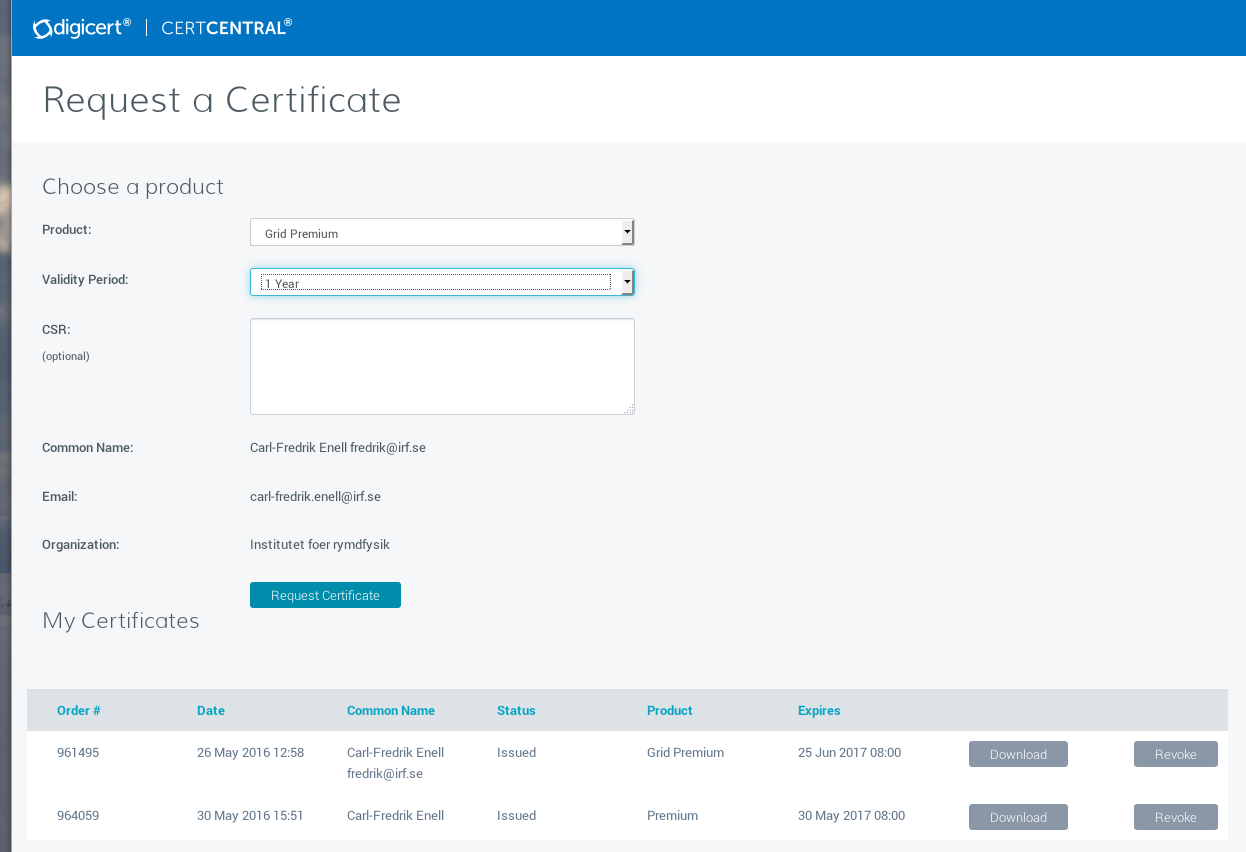
\includegraphics[width=1.0\linewidth]{digicert-request}
    \caption{Requesting a Grid Premium certificate from Digicert.}
    \label{fig:digicert}
  \end{figure}

\item If the Request procedure did not install the certificate
  automatically in your browser, it can be downloaded by looking up
  the new certificate in the list \emph{My certificates} and clicking
  the download button. This will give you a zip archive with your
  personal certificate together with a few other authority files. The
  certificate file (called something like \texttt{yourname.crt}) can
  then be imported.

  Fig.~\ref{fig:cert-browser} shows the details of the author's
  certificate after a successful import into Firefox.

  \begin{figure}[htb]
    \centering
     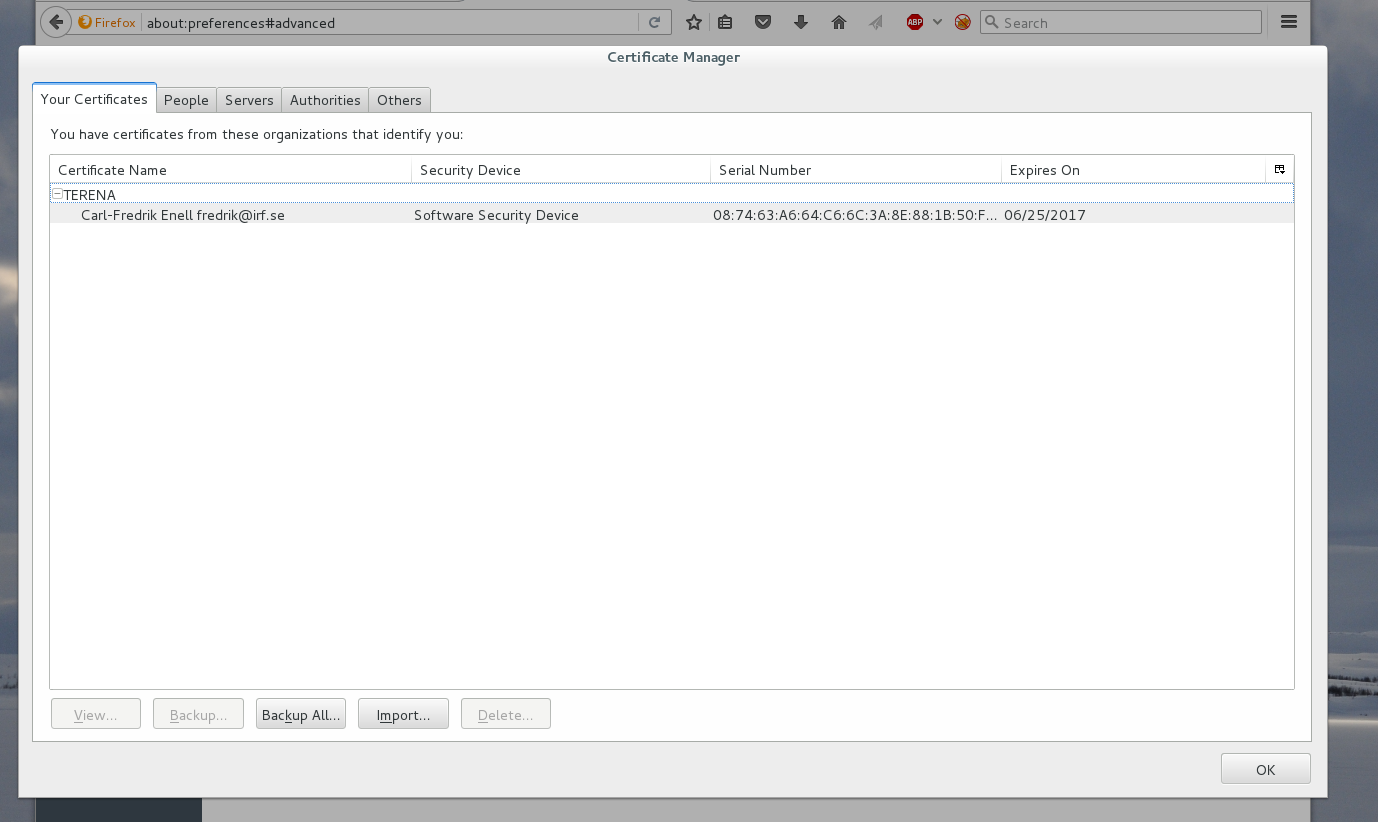
\includegraphics[width=1.0\linewidth]{cert-firefox}
    \caption{The certificate manager in Firefox (Edit $\rightarrow$ Preferences $\rightarrow$ Advanced $\rightarrow$ Certificates) after successfully importing a certificate from Digicert.}
    \label{fig:cert-browser}
  \end{figure}

\end{enumerate}

\subsubsection{Register Virtual Organisation membership}
\label{sec:regist-virt-organ}

\begin{enumerate}
  
\item Register to the \textbf{eiscat.se} VO through the \emph{Perun}
  service at
  \url{https://perun.metacentrum.cz/cert/registrar/?vo=eiscat.se}. You
  will have to enter required information and then wait for approval. Fig.~ shows a completed successful registration.

  \begin{figure}[htb]
    \centering
    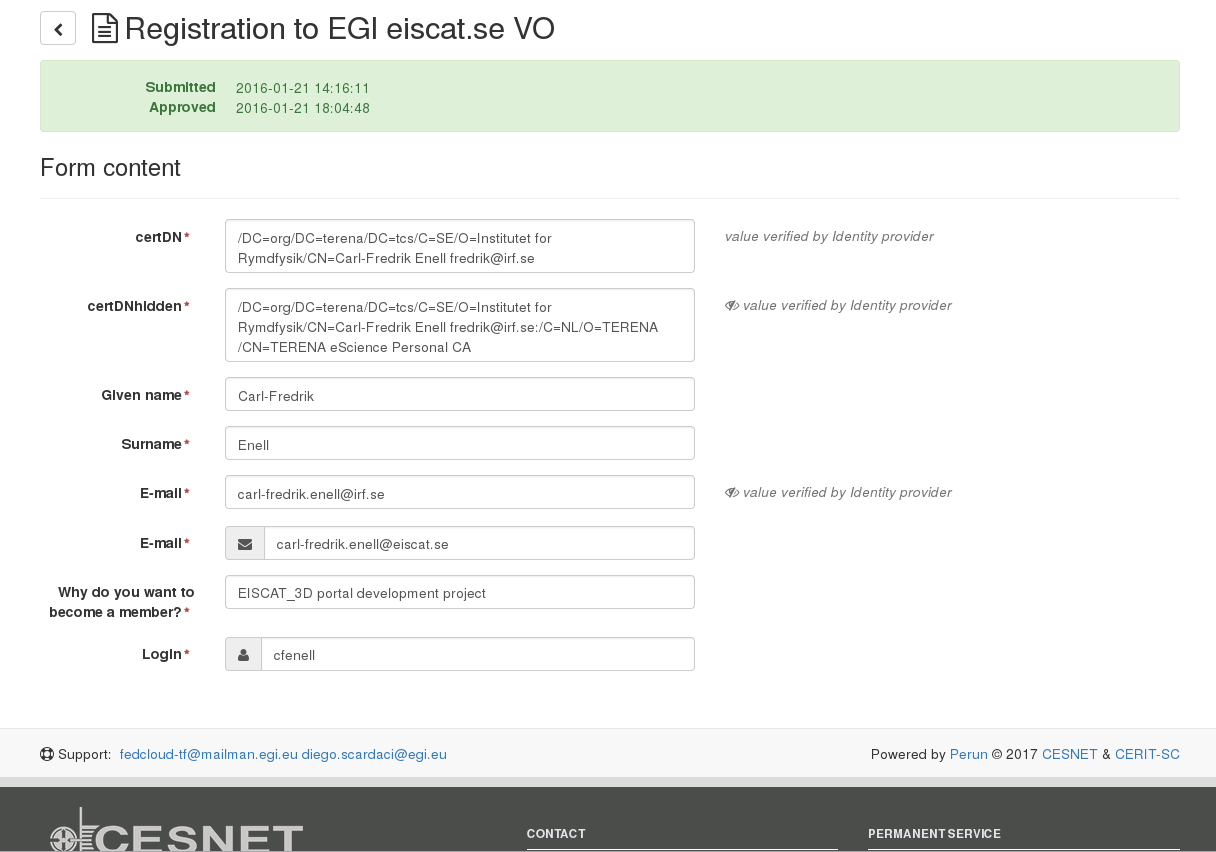
\includegraphics[width=1.0\linewidth]{perun-reg}
    \caption{Registration to the EGI VO \textbf{eiscat.se} through Perun.}
    \label{fig:perun-reg}
  \end{figure}


\item Ask a VO manager (e.g. the author) to add your VO user to the
  access groups that you are entitled to (usually your EISCAT
  associate country and common programme data). Fig.~\ref{fig:perun}
  shows the author editing access groups, and a similar
  procedure must be performed for your account.

\end{enumerate}

\subsubsection{Proxy upload}
\label{sec:proxy-upload}


\begin{enumerate}
  
\item Upload your certificate to the DIRAC proxy, which is the gateway
  that allows you to access the DIRAC grid services. This is easiest
  using the DIRAC command line tools. They are Python and UNIX (bash)
  shell scripts. If you cannot install them, the GUI also provides a proxy upload applet.

  \begin{figure}[htb]
    \centering
    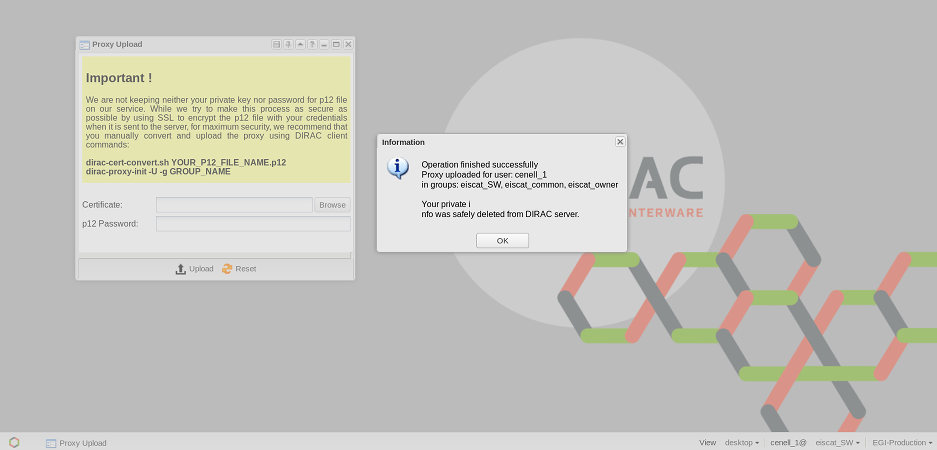
\includegraphics[width=1.0\linewidth]{dirac-gui-proxy}
    \caption{Proxy upload through the web GUI}
    \label{fig:proxygui}
  \end{figure}
  
  \begin{itemize}
  
  \item Export your certificate in p12 format. The export
    function of your web browser should work. This will ask you to
    set a password for encryption.

    
  \item Option 1: Use the web GUI (see Fig.~\ref{fig:proxygui}) to upload your certificate to the proxy.
    \begin{itemize}
    \item Select the Proxy upload applet in the web GUI
    \item Browse to your p12 format certificate
    \item Type in the password of the p12 certificate
    \item Click Upload
    \end{itemize}

  \item Option 2: Use the DIRAC CLI to install the certificate for the DIRAC services and upload to the proxy.  Refer to \url{http://diracgrid.org} for instructions on how to install the DIRAC client or run it in a Docker container.

    \begin{verbatim}
     dirac-cert-convert.sh <YOUR_CERTIFICATE>.p12
     \end{verbatim}

  \item Upload the certificate and initialise the DIRAC proxy:

\begin{verbatim}
      dirac-proxy-init -M -U -g eiscat_<GROUP>
\end{verbatim}

    for example:
\begin{verbatim}
      dirac-proxy-init -M -U -g eiscat_FI
\end{verbatim}
    
    
    You will be asked for the password of your certificate (the one you set in the export step above).
    You can then check whether the upload succeeded like this:
    \begin{verbatim}
      dirac-proxy-get-uploaded-info 
    \end{verbatim}

    and you should then see something like
  \end{itemize}


\noindent
{\tiny
\begin{verbatim}
Checking for DNs /DC=org/DC=terena/DC=tcs/C=SE/O=Institutet foer rymdfysik/CN=Carl-Fredrik Enell fredrik@irf.se
-------------------------------------------------------------------------------------------------------------------------------------------------------------------
| UserName | UserDN                                                                                         | UserGroup    | ExpirationTime      | PersistentFlag |
----------------------------------------------------------------------------------------------------------------------------------------
| cenell_1 | /DC=org/DC=terena/DC=tcs/C=SE/O=Institutet foer rymdfysik/CN=Carl-Fredrik Enell fredrik@irf.se | eiscat_SW    | 2017-06-25 11:54:59 | True           |
-------------------------------------------------------------------------------------------------------------------------------------------------------------------
\end{verbatim}
}%tiny

\end{enumerate}



\begin{figure}[htb]
  \centering
  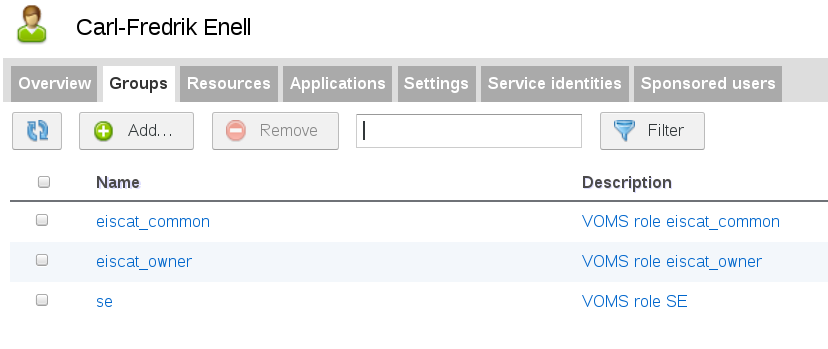
\includegraphics[width=1.0\linewidth]{voms-groups-perun}
  \caption{The Groups tab of the Perun VOMS GUI, showing access groups of the author. This registration will be handled by one of the VO managers so as a normal user you will not see this. It is important that you are a member of the appropriate VOMS group(s), however.}
  \label{fig:perun}
\end{figure}


To connect to the web GUI, browse to
\url{https://dirac.egi.eu:9443/DIRAC/}. The browser may ask you to use
the installed certificate. If not, click the label ``Visitor'' at the
bottom left and choose certificate authentication.


\subsection{EGI Checkin authentication}
\label{sec:checkin-auth}

It has turned out that the project needs an optional authentication
mechanism to account for users who do not have access to certificates
or work outside Europe. EOSC-Hub offers three options, originating from EGI (Checkin), EUDAT (B2ACCESS) and Indigo (IAM) respectively. These can all work with several identity providers, and we chose EGI Checkin for the DIRAC portal. This type of authentication has now been implemented.

To authenticate with EGI Checkin, follow these simple steps:

\begin{enumerate}
  
\item Connect to the EISCAT DIRAC portal at
  \url{https://dirac.egi.eu:9443/DIRAC/}. If you don't have a
  certificate, the login selector in the lower right corner will show
  ``Visitor''.

\begin{figure}[htb]
  \centering
  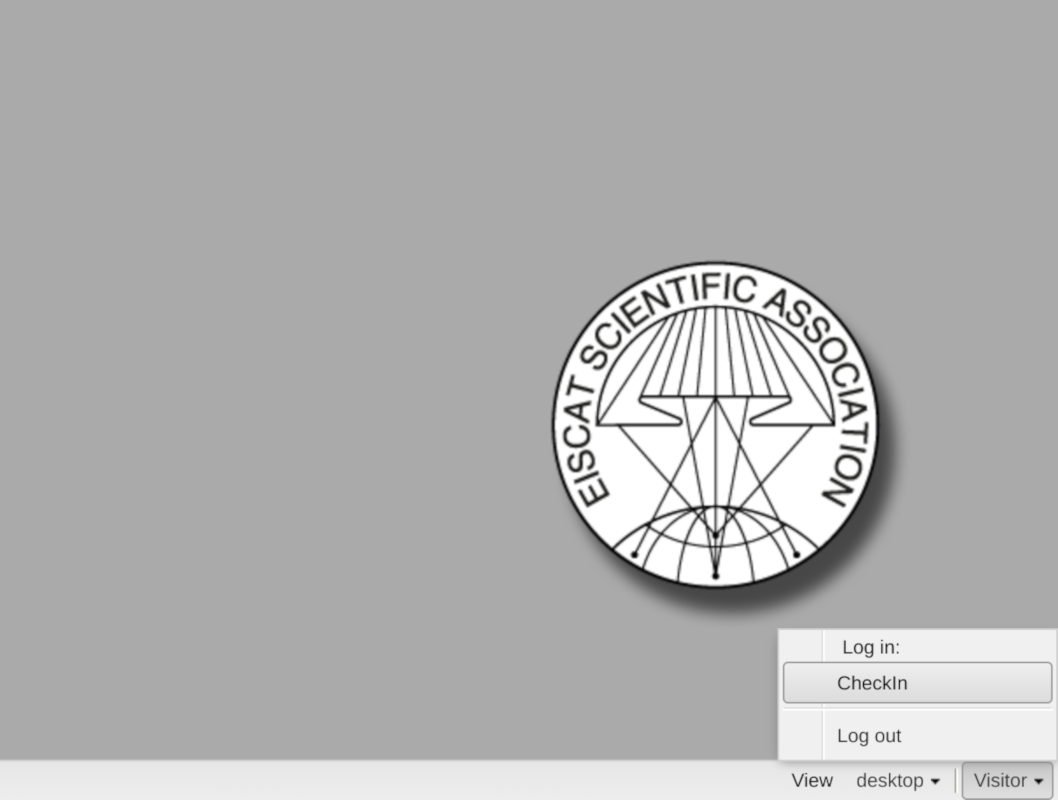
\includegraphics[width=0.5\linewidth]{dirac-gui-checkin}
  \caption{Selecting the EGI Checkin login option in the DIRAC Web GUI.}
  \label{fig:checkin}
\end{figure}

  
\item Select the EGI Checkin login option, as shown in Fig.~\ref{fig:checkin}.
Checkin will allow you to select an identity provider, which handles the actual login. Options include EduGAIN and social media accounts.

\item The identity provider will send the credentials back to Checkin,
  and you will have to accept this.

\begin{figure}[htb]
  \centering
  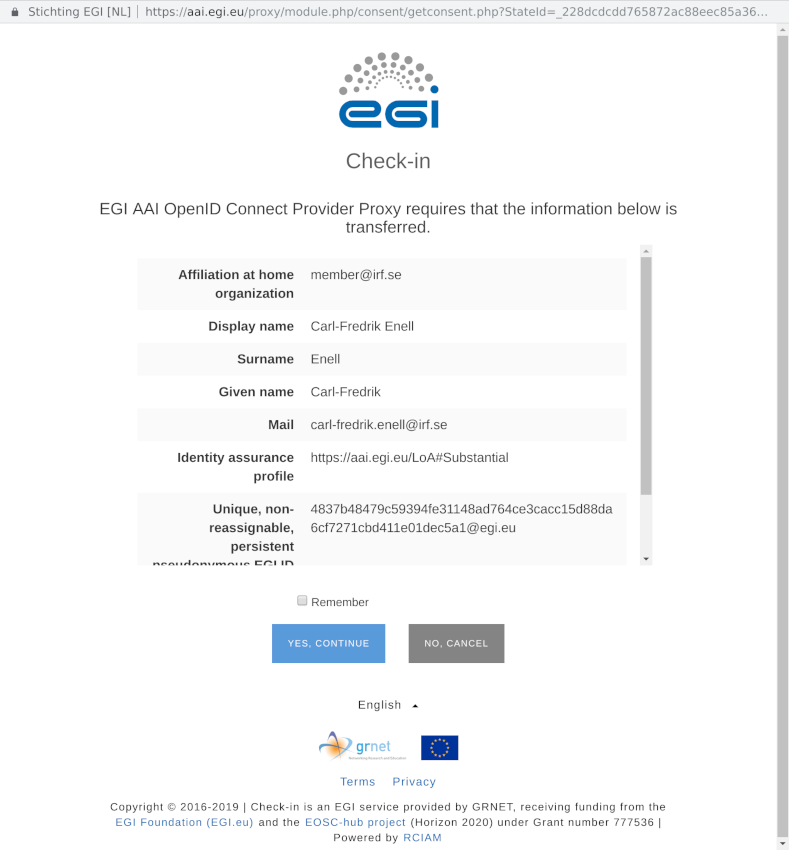
\includegraphics[width=0.5\linewidth]{checkin-accept}
  \caption{After successfully logging in to the identity provider, EGI Checkin will require permission to transfer the required information. Click Accept on this page.}
  \label{fig:checkin}
\end{figure}

\end{enumerate}


\section{Searching EISCAT data}
\label{sec:searching}

Once authenticated you can start using the web GUI. The text ``Visitor'' should now have changed to ``EGI Production'', and selectors for user name(s) and granted VOMS access groups will appear, as shown in Fig.~\ref{fig:checkin-succeeded}.

\begin{figure}[htb]
  \centering
  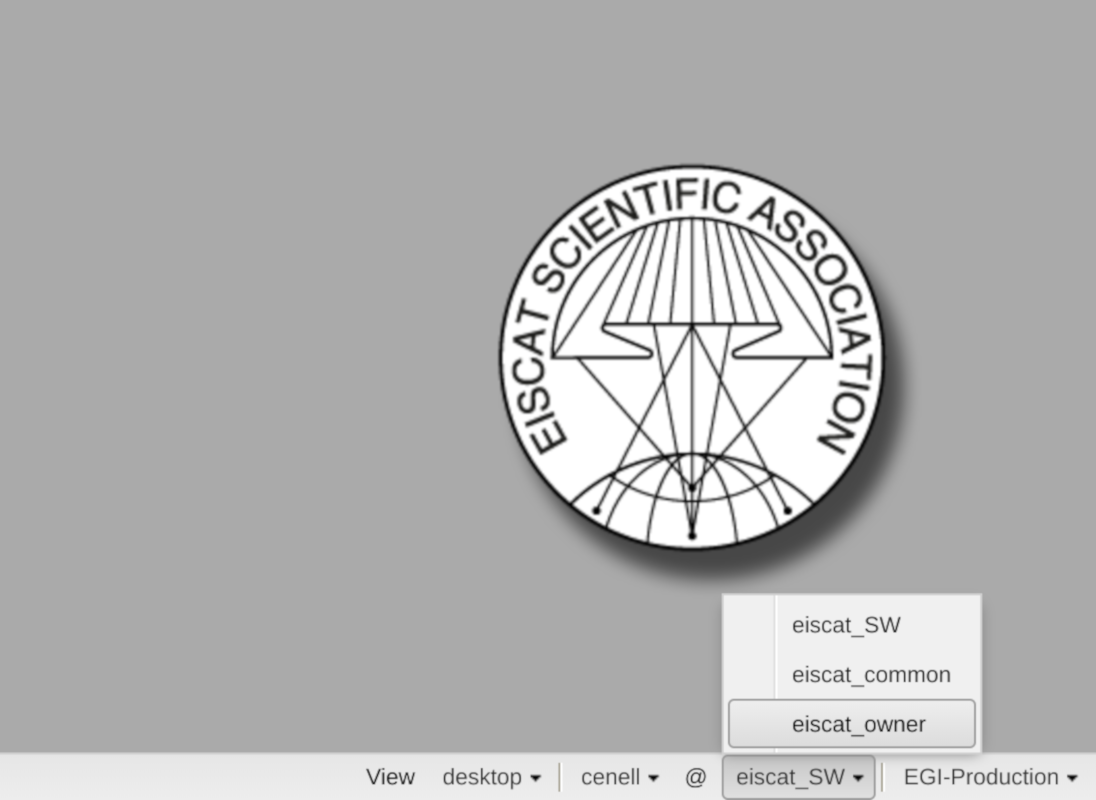
\includegraphics[width=0.5\linewidth]{dirac-gui-checkin-ok}
  \caption{Successfully logged in to the DIRAC portal. The lower right text will change from ``Visitor'' to ``EGI Production'' and the user can select access groups in which membership has been granted.}
  \label{fig:checkin-succeeded}
\end{figure}

The point of start in the portal is the file catalogue GUI. To access it:

\begin{enumerate}
\item Connect and authenticate as described
\item Select your VOMS group, such as \texttt{eiscat\_SE}
\item Go to the Windows style menu at the bottom left and browse to the file catalogue GUI. 
\end{enumerate}

\subsection{Basic search}
\label{sec:searchdir}


\begin{itemize}
\item  The file catalogue GUI will look much like any file browser. The search will, however, start from a top level directory that you select by right-clicking on a directory in the listing (top right pane) and then clicking \texttt{Set as starting path} (See Fig.~\ref{fig:catalogue}). EISCAT data are in the directory hierarchy \texttt{eiscat.se/archive/<year>/}.
\item After setting the starting path, additional search criteria can be added using the GUI in the top left pane. See Fig.~\ref{fig:search}. 
\item Click Submit (below the bottom left pane). 
\end{itemize}

\begin{figure}[htb]
  \centering
  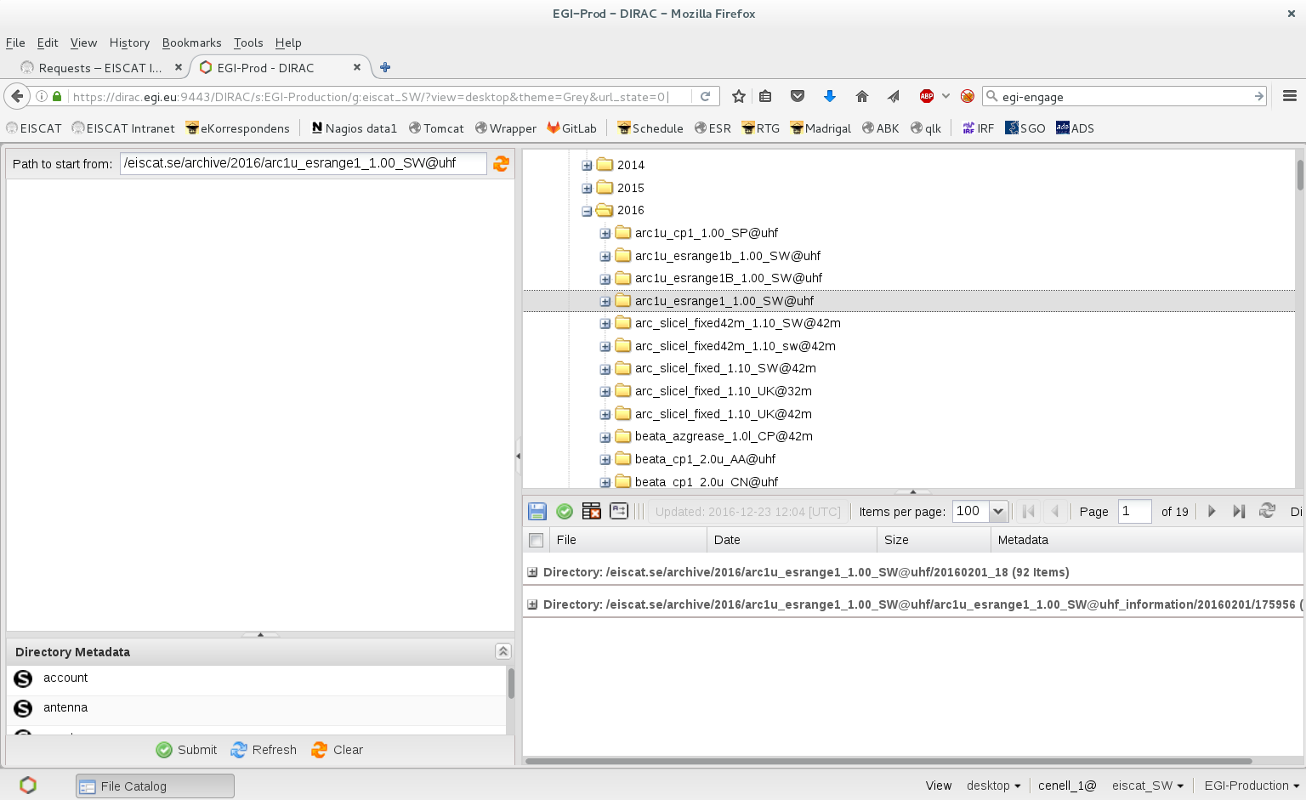
\includegraphics[width=1.0\linewidth]{dirac-gui-catalogue}
  \caption{Selecting a top level directory in the file catalogue GUI}
  \label{fig:catalogue}
\end{figure}

\begin{figure}[htb]
  \centering
  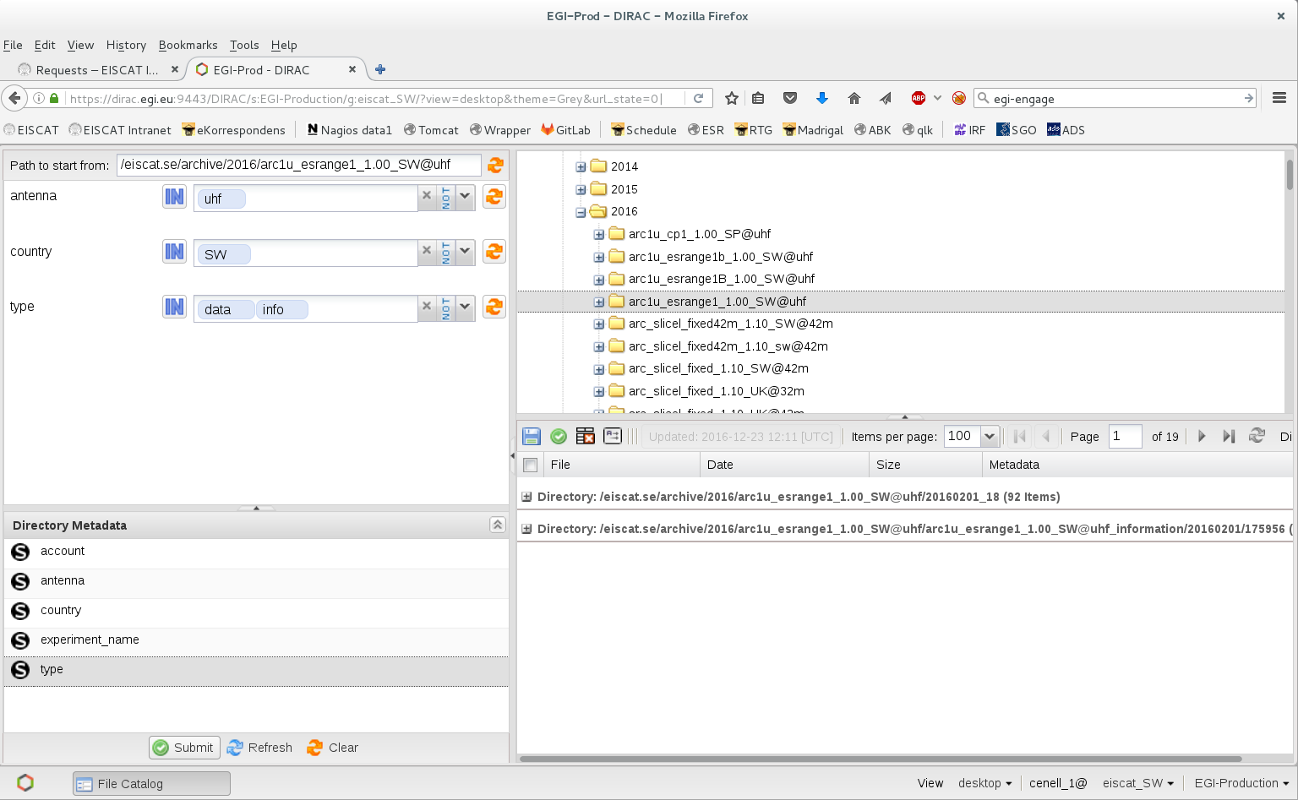
\includegraphics[width=1.0\linewidth]{dirac-gui-search}
  \caption{Adding metadata search criteria. In this particular case, the top level directory contains only SW UHF data, so the filters shown as an example on the top left will have no effect. After selecting the search criteria, click the Submit button}
  \label{fig:search}
\end{figure}


The search will list any found files in the bottom right pane.  After
finding the desired files, you can select files for download or
processing in the bottom right pane.

\section{Downloading EISCAT data}
\label{sec:download}


Files selected in the bottom right pane can be downloaded as a ZIP
archive by clicking on the diskette icon, as shown in
Fig.~\ref{fig:download}.
\begin{figure}[htb]
  \centering
  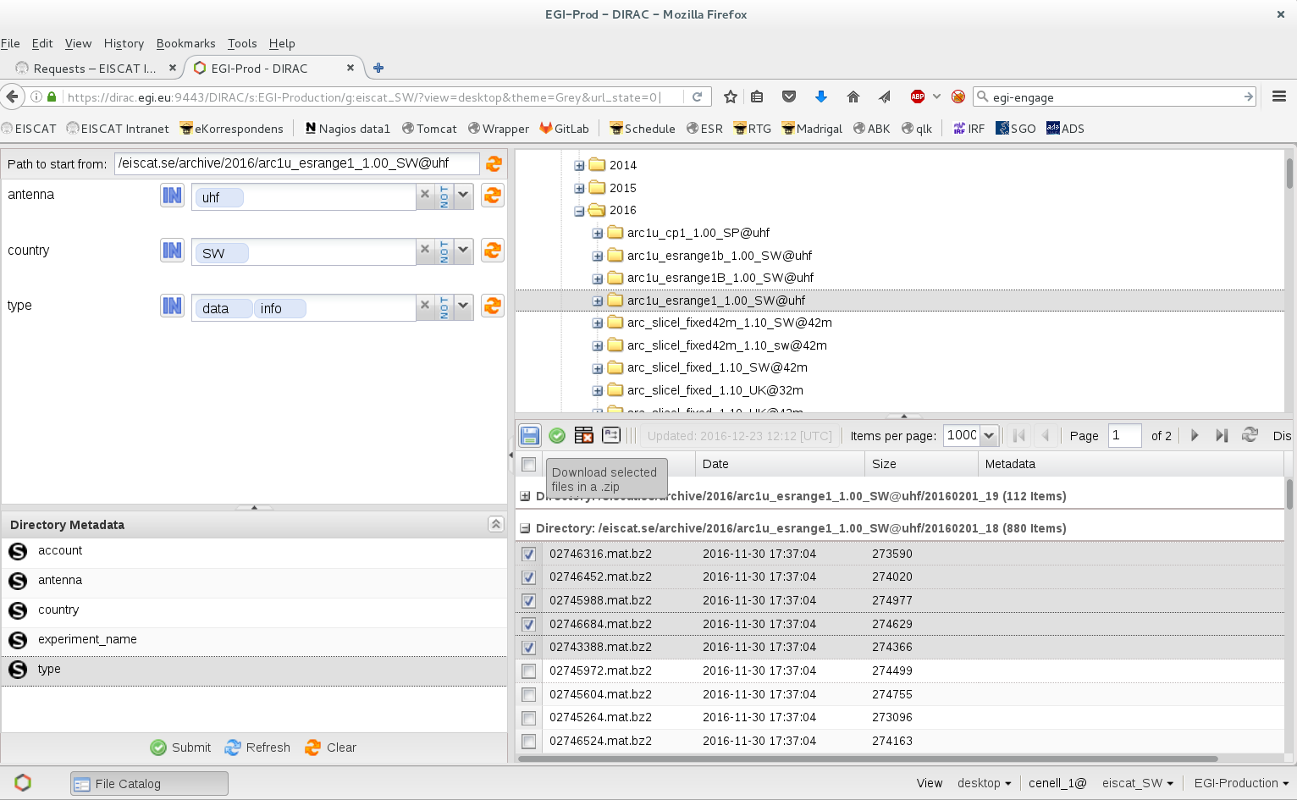
\includegraphics[width=1.0\linewidth]{dirac-gui-download}
  \caption{Selecting files to download.}
  \label{fig:download}
\end{figure}

\section{Submitting user analysis jobs}
\label{sec:rtg}

\subsection{Using the Job Launchpad GUI}
\label{sec:using-job-launchpad}

The GUI can also submit processing jobs. This procedure will essentially

\begin{enumerate}
\item start a pilot job on the compute resources

\item the pilot job downloads and runs the specified software with the
  selected files as input.
\end{enumerate}

At this stage the standard EISCAT Real Time Graph (RTG) has been
implemented and will plot the content of the selected data files (by
running the RTG script on the open source Matlab-compatible software
Octave).


The Job Launchpad is a separate application in the GUI, but it can also be accessed from the file catalogue as follows:
\begin{enumerate}
\item Select files in the same way as for download
\item Click the green job launchpad icon above the file list
\item The job launchpad GUI should open. Right-click on the \texttt{EISCAT png maker} directory icon and select \texttt{Apply to the selected parameters}. See Fig.~\ref{fig:submit}.
The field \texttt{Executable} should now show the path to \texttt{webtg4dirac}.
\item Check the other parameters as well and click Submit at the bottom of the job launchpad window.
\item Go to the main menu and browse to the job monitor (Fig.~\ref{fig:monitor}). Make sure that your user name is preselected and click Submit to see the status of the job.
\item Once the job is finished, the output will be in the Sandbox. Right-click on the job line to see the menu as in Fig.~\ref{fig:sandbox}.
\end{enumerate}


\begin{figure}[htb]
  \centering
  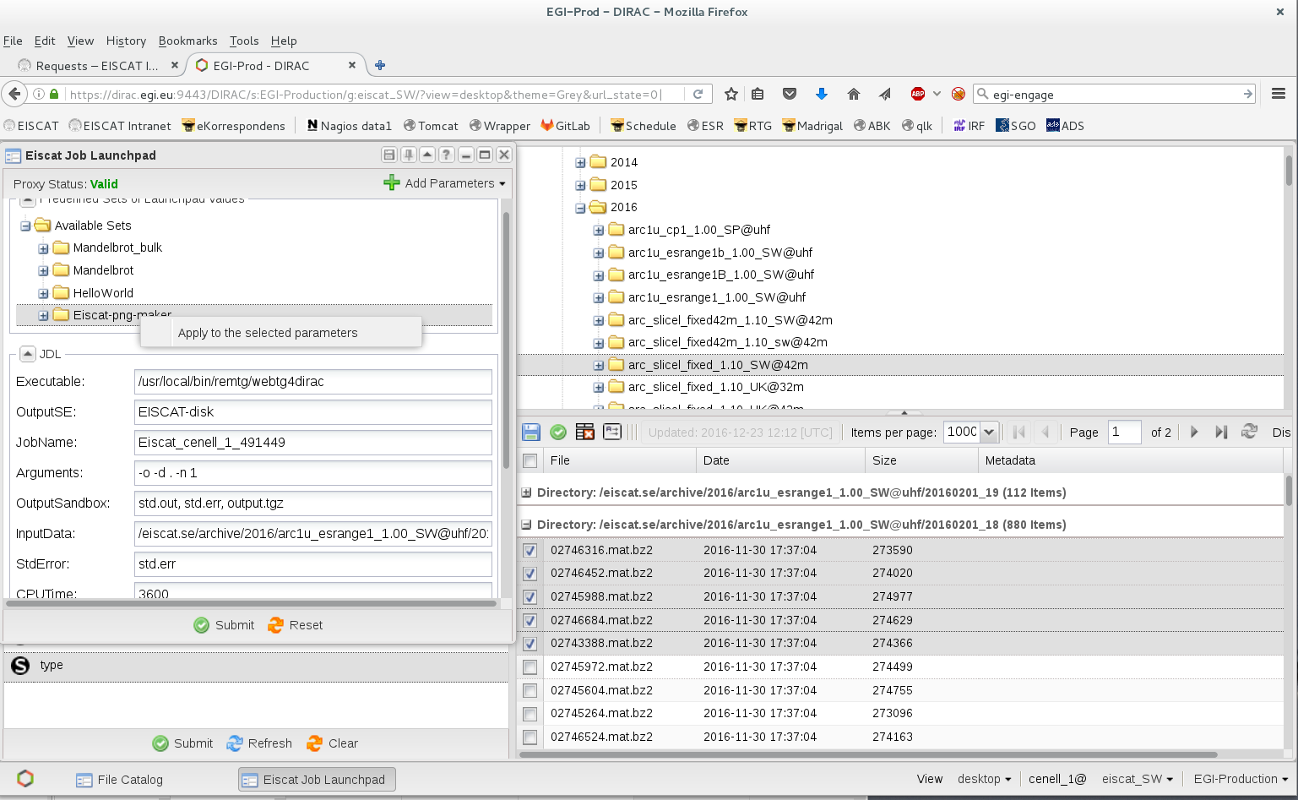
\includegraphics[width=1.0\linewidth]{dirac-gui-jobsubm}
  \caption{Submitting a job that will plot the selected EISCAT data files with RTG.}
  \label{fig:submit}
\end{figure}

\begin{figure}[htb]
  \centering
  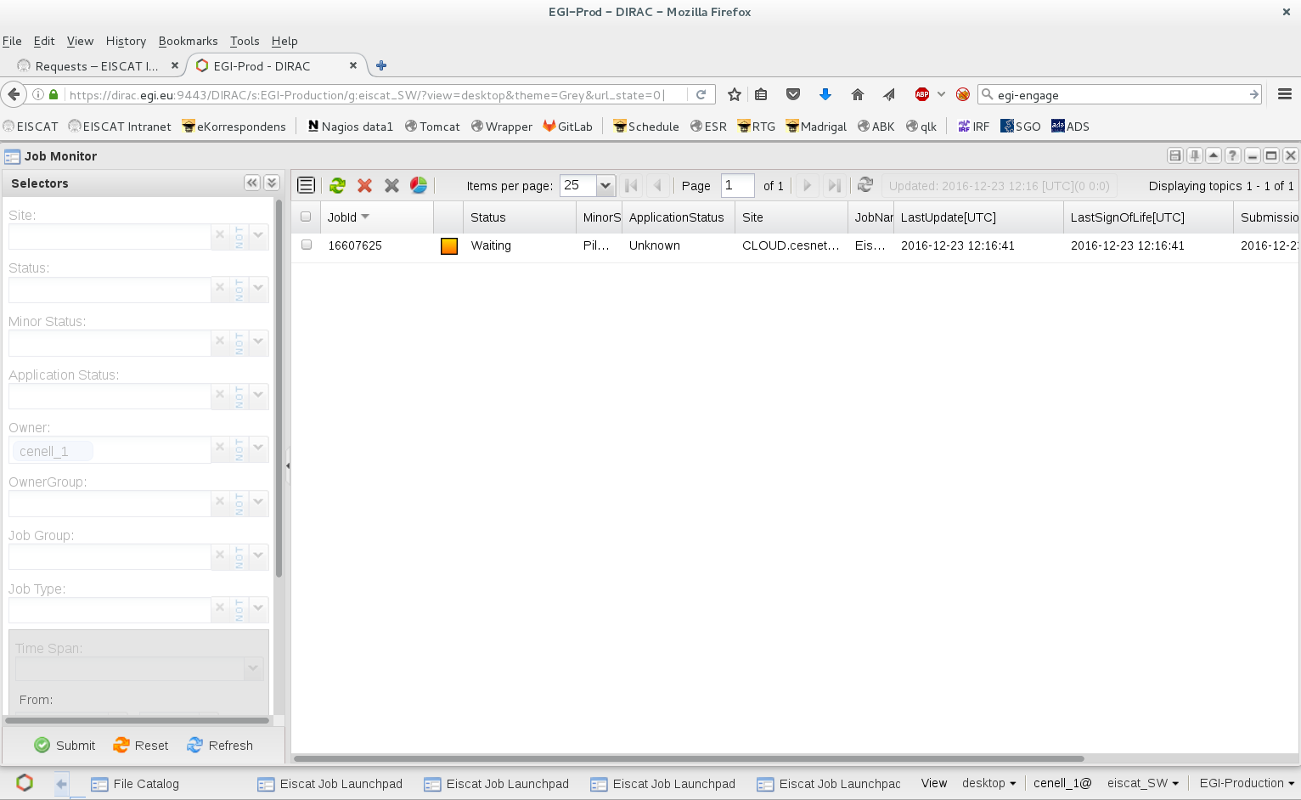
\includegraphics[width=1.0\linewidth]{dirac-gui-jobmon}
  \caption{The DIRAC job monitor showing the status of the submitted job.}
  \label{fig:monitor}
\end{figure}

\begin{figure}[htb]
  \centering
  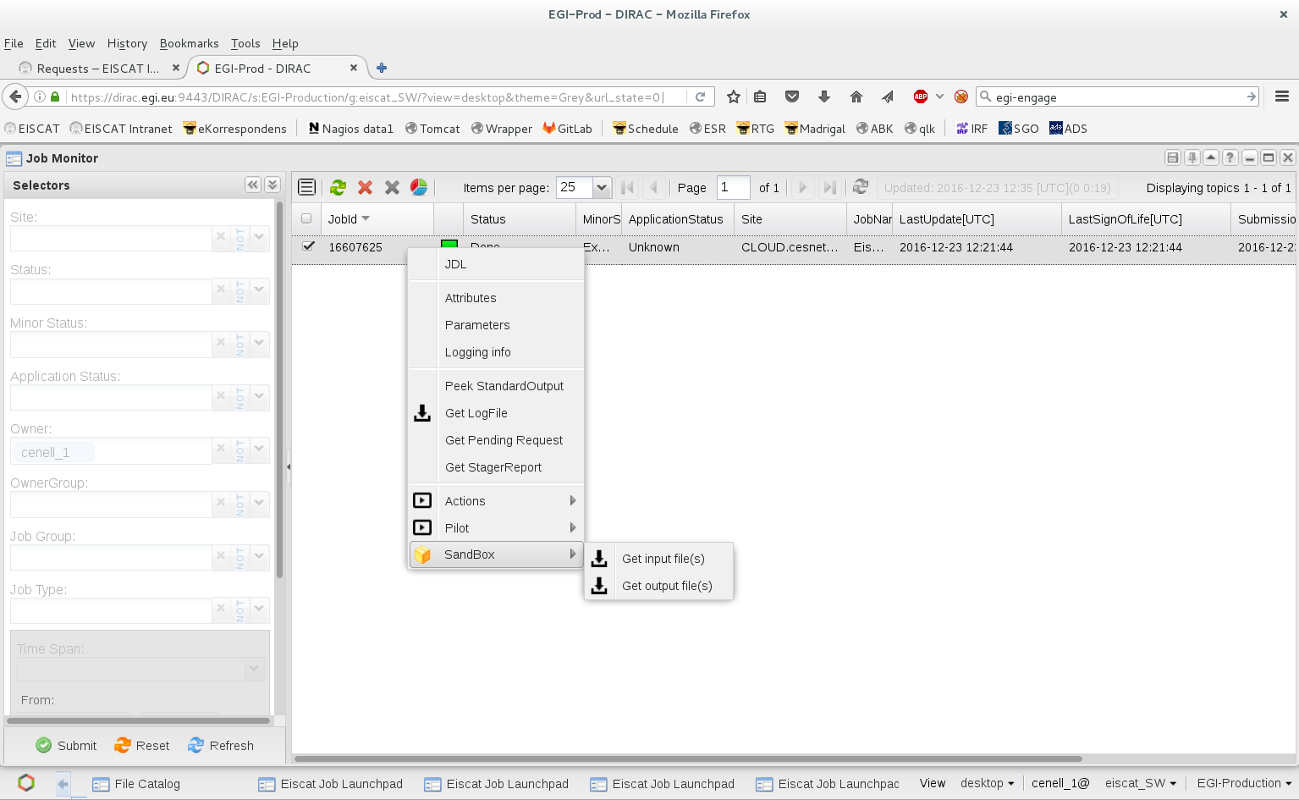
\includegraphics[width=1.0\linewidth]{dirac-gui-job-get}
  \caption{The sandbox contains the output files for download.}
  \label{fig:sandbox}
\end{figure}

\subsection{Using the CLI}
\label{sec:using-cli}

Jobs can also be submitted from the DIRAC command line. For this, a job description file has to be written and submitted. A typical job description file has this format, known as JDL (Job Description Language):

\begin{verbatim}
 
[
      Executable = "run_rtg_docker.sh";
      Arguments = "";
      JobName = "my_job_name_string";
      Site = "Cloud.CSC.fi";
      CPUTime = 86400;
      InputSandbox = {"run_rtg_docker.sh",
            "LFN:/eiscat.se/archive/yyyy/experiment/file1",
            "LFN:/eiscat.se/archive/yyyy/experiment/file2",
            ...
           }
      OutputSandbox = {"output/*"};
    ]


  
\end{verbatim}

The principle of job submission through the CLI is thus:

\begin{description}
\item Edit and save a JDL file for your analysis case, e.g. \verb+my_job.jdl+.
  
\item Submit the job: \verb+dirac-wms-job-submit my_job.jdl+

\end{description}

For further instructions, please refer to the instructions at
\url{https://dirac.readthedocs.io/en/latest/UserGuide/index.html}

\section{Feedback}
\label{sec:feedback}
Feedback and bug reports through the EGI RT tracker system will be appreciated. EISCAT portal reports should be submitted through
 \url{https://rt.egi.eu/rt/Search/Results.html?Query=Queue\%20\%3D\%20\%27dirac4egi-eiscat3d-requirements\%27\%20AND\%20(Status\%20\%3D\%20\%27new\%27\%20OR\%20Status\%20\%3D\%20\%27open\%27\%20OR\%20Status\%20\%3D\%20\%27accepted\%27\%20OR\%20Status\%20\%3D\%20\%27developed\%27\%20OR\%20Status\%20\%3D\%20\%27stalled\%27\%20OR\%20Status\%20\%3D\%20\%27feedback\%27)}.

\end{document}

%%% Local Variables:
%%% mode: latex
%%% TeX-master: t
%%% End:
